\chapter{Umsetzung}

%was wurde wie umgesetzt, was nicht und warum!? - problemstellungen..

Bei der Umsetzung wurde versucht die Eigenheiten von Unity zu nutzen eine einfache und Anpassbare Engine f�r Behaviourtrees zu entwickeln.\\
Die Engine besteht im Kern 2 Klassen die Abstrakt sind. Aus diesen lassen sich alle ben�tigten knoten ableiten.
Zus�tzlich gibt es noch eine Verwalter-Klasse.

F�r die Visuelle Darstellung wurde ein MVC eingesetzt. Wobei leider regeln des MVC gebrochen werden mussten da es keine einfache M�glichkeit gab an die entsprechenden variablen und Funktionen zu gelangen.

\section{Kern-Klassen}
 Zur Feststellung der Vater-Kind-Beziehungen von Knoten wird die Struktur von Unity benutzt da diese schon zur Verf�gung steht. Dies erlaubt es Entwicklern auch ohne Editor funktionierende Verhaltensb�ume zu bauen und modifizieren.
\subsection{BehaviourNode}
\begin{figure}[h!] %[hbtp]
	\centering
		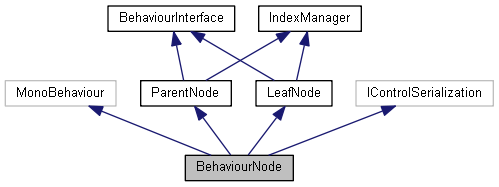
\includegraphics[width=0.5\textwidth]{images/class_behaviour_node__coll__graph.png}
	\caption{Beziehung der BehaviourNode Klasse}
	\label{a1}
\end{figure}
\textbf{BehaviourNode} ist die eine abstrakte Klasse auf der alle Inneren Knoten wie \textbf{Selector}, \textbf{Sequence} oder \textbf{UtilFail} basieren. Falls ein weiterer Innerer Knoten ben�tigt wird empfiehlt es sich von dieser Klasse abzuleiten.
\newpage
\subsection{Task}

\begin{figure}[h!] %[hbtp]
	\centering
		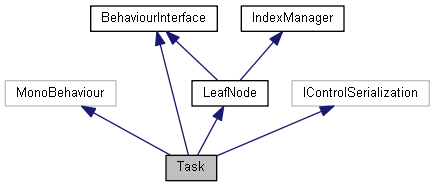
\includegraphics[width=0.5\textwidth]{images/class_task__coll__graph.png}
	\caption{Beziehung der Task Klasse}
	\label{a2}
\end{figure}
Die abstrakte Klasse \textbf{Task} ist die Basis aller Tasks die vom Baum ausgef�hrt werden k�nnen. Sie ist so angelegt das ein Task keine weiteren Kind-Knoten haben kann. Wie ein neuer Tasknode aussehen kann l�sst sich gut an den Beispielklassen \textbf{OutputTask} und \textbf{WaitTimeTask} erkennen.

\subsection{BehaviourTree}

\begin{figure}[h!] %[hbtp]
	\centering
		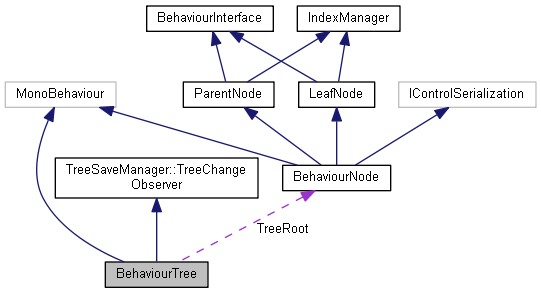
\includegraphics[width=0.5\textwidth]{images/class_behaviour_tree__coll__graph.png}
	\caption{Beziehung der BehaviourTree Klasse}
	\label{a3}
\end{figure}
\textbf{BehaviourTree} Stellt die Schnittstelle zwischen Verhaltensbaum und Spielobjekt da. Der \textbf{Owner}(Eigent�mer) des Baumes und kann ein Beliebiges \textbf{GameObject} sein. Auf diesen k�nnen w�hrend der Laufzeit \textbf{Tasks} und \textbf{BehaviourNodes} zu greifen. 

\section{Editor}
Das GUI f�r die Bearbeitung der Behaviourtrees wurde mit Hilfe von NGUI erstellt.\\
NGUI ist eine m�chtige Erweiterung f�r Unity die es erm�glicht komplexe und dynamische GUI's zu erstellen.
\subsection{TreeVis}
\begin{figure}[h!] %[hbtp]
	\centering
		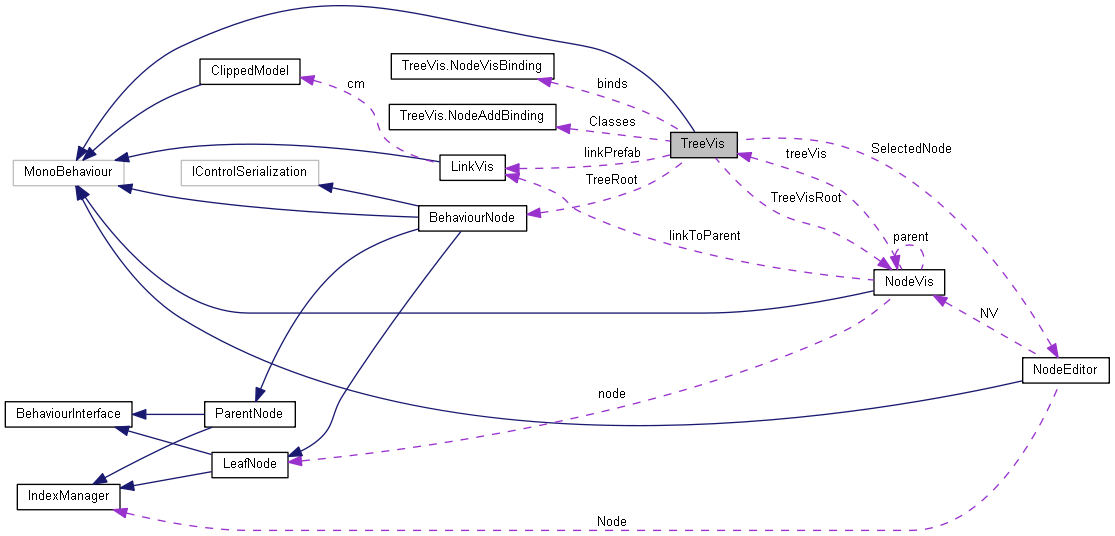
\includegraphics[width=0.5\textwidth]{images/class_tree_vis__coll__graph.png}
	\caption{Beziehung der TreeVis Klasse}
	\label{a4}
\end{figure}
\textbf{TreeVis} ist das Kernst�ck zum Visualisieren eines Behaviourtrees. Diese Klasse startet eine Rekursive Generierung des Visuellen Baumknoten. Welches UIPrefab f�r einen Knoten verwendet wird kann der Nutzer �ber die TreeVis Instanz im Unity Editor festlegen. Auch welche Knoten Hinzugef�gt werden k�nnen, kann der Nutzer festlegen.

\subsection{NodeVis}
Die Klasse \textbf{NodeVis} k�mmert sich um die Richtige Positionierung und anzeigen des Statutes des Knoten.

\subsection{NodeEditor}
Die \textbf{NodeEditor} Klasse hingegen ist f�r die Ver�nderung von den Knoten zust�ndig wie Position in der Baumebene oder Erstellen neuer Kind-Knoten. Diese ist die Abstrakte Vaterklasse von \textbf{BehaviourEditor} und \textbf{TaskEditor}

\subsection{TaskAttributes}
Da der Nutzer die M�glichkeit haben sollte Attribute von bestimmten Tasks zu ver�ndern, musste ein System geschaffen werden das es erlaubt Attribute die ver�ndert werden k�nnen anzumelden.
Um eine Kommunikation zwischen UI und Klasse zu erm�glichen kann der Entwickler einen Setterfunktion f�r die Variablen anmelden. Momentan werden \textbf{FLOAT}, \textbf{INT}, \textbf{BOOL} und \textbf{STRING} unterst�tzt. Ein Beispiel f�r die Verwendung eines \textbf{STRING} kann in der \textbf{OutputTask} Klasse gefunden werden.